\section{Misurazione della pressione di vapore dell'acqua a temperature differenti}

In questa sezione illustreremo il materiale a nostra disposizione per l'esecuzione
dell'esperimento e di seguito faremo un'analisi dei dati da noi raccolti.

\subsection{Apparato sperimentale}

Il materiale a nostra disposizione è il seguente:
\begin{itemize}
	\item{Riscaldatore con agitatore magnetico;}
	\item{Termometro ad alcohol con una risoluzione di misura di 1$^\circ$C;}
	\item{Manometro di Bourdon con una risoluzione di misura di 5000 Pa;}
	\item{Apparato per la misura della pressione di vapore, consistente in un beaker,
    in una bottiglietta di vetro con tappo sigillante, un sostegno per l'apparato, acqua distillata e raccorderia varia;}
\end{itemize}

\begin{figure}[b!]
    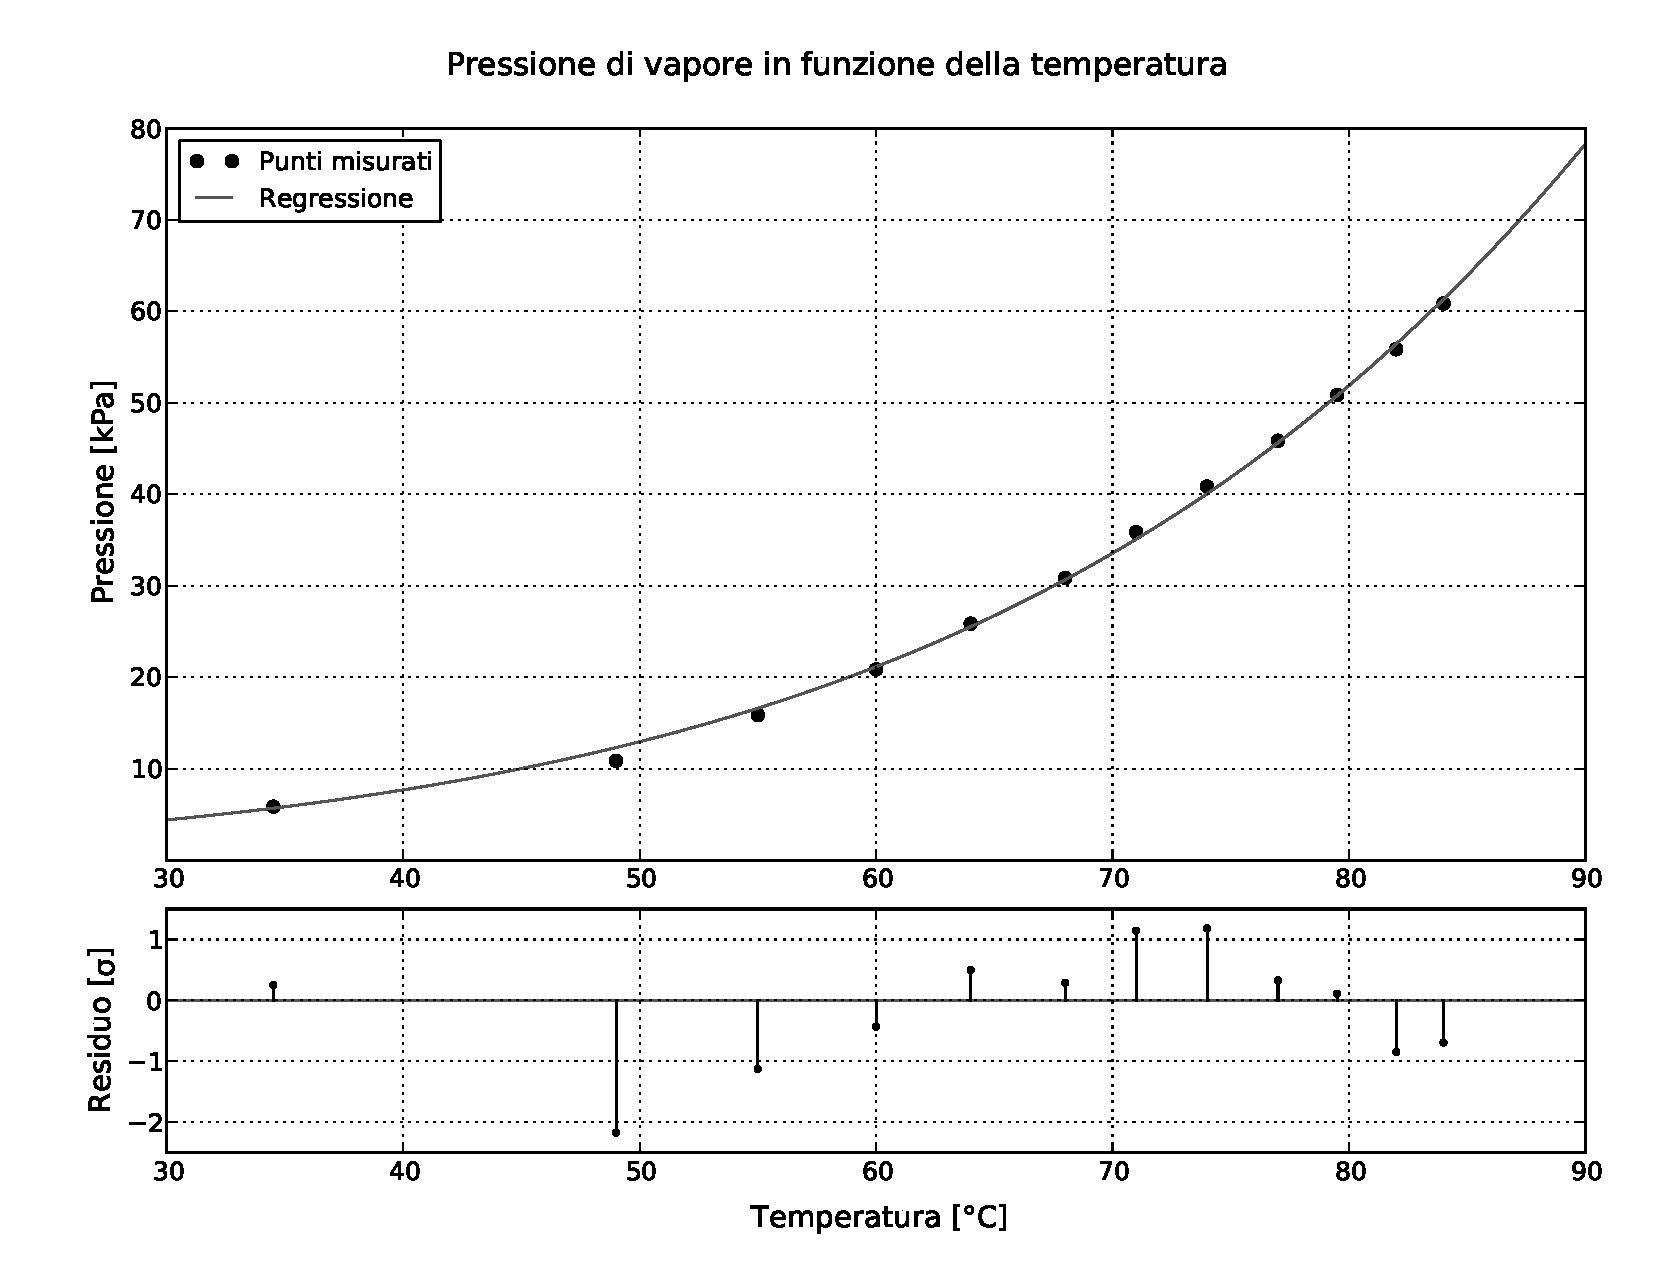
\includegraphics[width=17cm]{graph.pdf}
    \caption{Il grafico mostra i dati raccolti con la relativa incertezza. I dati seguono bene
    l'andamento tipico della pressione di vapore in funzione della temperatura.
    La curva tracciata è stata ottenuta con il metodo dei minimi quadrati.}
    \label{fig:graph}
\end{figure}

\subsection{Raccolta dati}

Per misurare la pressione di vapore dell'acqua a differenti temperature abbiamo adottato questo procedimento:

\begin{itemize}
	\item{abbiamo posto a bagnomaria la bottigietta di vetro;}
	\item{abbiamo fatto rggiungere la temperatura di circa 20$^\circ$C all'acqua demineralizzata interna alla bottiglietta;}
	\item{variando la pressione interna della bottiglietta abbiamo riempito il
        tubicino che collega la bottiglia con il manometro di acqua, che è un fluido incomprimibile;}
	\item{una volta che il sistema ha raggiunto la temperatura di 35$^\circ$C abbiamo
        iniziato a raccogliere i dati leggendo per ogni variazione della pressione pari
        a 5 kPa, la corrispettiva temperatura dell'acqua nella bottiglia;}
	\item{il processo è stato interrotto una volta raggiunta una temperatura interna di
        circa 85$^\circ$C. A questo punto non si è più somministrata energia al sistema e sono
        stati raccolti i dati in discesa, ovvero man mano che il sistema andava raffreddandosi;}
\end{itemize}

\subsection{Analisi dei dati}

